\documentclass{article}

\usepackage[xetex]{graphicx}
\usepackage{subfig}
\usepackage{float}
\graphicspath{{picture/}}
\usepackage[colorlinks]{hyperref}

\newtheorem{definition}{definition}[section]
\newtheorem{property}{property}[section]

\begin{document}
\title{A Brief Introduction of Self-balancing Trees}
\author{Stephen Yang}
\date{July, 2023}
\maketitle

\tableofcontents


\newpage
\section{Introduction}

\subsection{Tree}

\begin{definition}
    In graph theory, a tree is an undirected graph in which any two vertices are connected by exactly one path or, equivalently, a connected acyclic undirected graph.
\end{definition}

\paragraph{}
Trees can help humans to organize the relationship between the data, but for most trees, it's pretty hard for a computer to understand and deal with. However, we have some specific trees with specially designed structures so that computers can interact with data quickly with them.

\paragraph{}
This essay will discuss these tree structures' concepts and how they are implemented. Some comparison of their performance, as well as their applications in real life, would also be included.

\subsection{Binary Search Tree (BST)}

\begin{definition}
    A binary tree is a tree data structure in which each node has at most two children, the left and right child.
\end{definition}

\paragraph{}
A binary tree is a structure with great potential. It's easy for a computer to represent with a handful of memory. More importantly, storing data in a specific order to a binary tree makes searching for the data later in it easy.

\begin{definition}
    In computer science, a binary search tree (BST), also called an ordered or sorted binary tree, is a rooted binary tree data structure with the key of each internal node being greater than all the keys in the respective node's left subtree and less than the ones in its right subtree. 
\end{definition}

\paragraph{}
With a BST, binary search algorithm can be used to search data. In the best situation, we only need $O(\log{N})$ time to get the result. With the same data, BST's height is expected to be as short as possible, which means it should be as bushy as possible.

But here's a problem. Consider adding 1 to 7 into a BST. By adding them in ascending order, we get BST shown in figure~\ref{spindlyBST}. By adding numbers in the order of $4,2,6,1,3,5,7$, we get BST shown in figure~\ref{bushyBST}. It's easy to find that The worse query time complexity for BST \ref{spindlyBST} is $O(N)$, for BST \ref{bushyBST} is $O(\log{N})$.

\begin{figure}[htbp]
    \centering

	\begin{minipage}{0.49\linewidth}
		\centering
		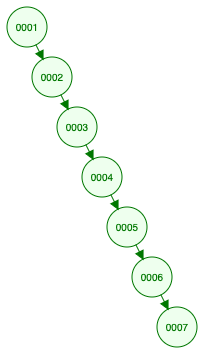
\includegraphics[height = 100 pt]{spindlyBST.png}
		\caption{BST1}
		\label{spindlyBST}
	\end{minipage}
	\begin{minipage}{0.49\linewidth}
		\centering
		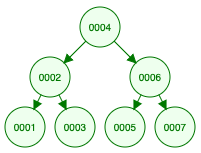
\includegraphics[height = 100 pt]{bushyBST.png}
		\caption{BST2}
		\label{bushyBST}
	\end{minipage}

\end{figure}
\newpage

\paragraph{}
If the data are inserted randomly, the query time complexity is $O(\log{n})$. But if a data set is inserted in ascending/descending order to a BST, the tree would degenerate into a linked list.

In daily life, many data are well-organized, so if we directly add them into a BST, the tree would be pretty spindly, which leads to a bad performance. Therefore, some trees which can avoid this situation are required.

\newpage


\section{Self-Balancing Tree}
\paragraph{}
This section will introduce several kinds of self-balancing trees; they are designed to avoid the appearance of very bad structures. Some have special construction, and some use a special operation called tree rotation(\ref{rotation}) to transform a spindly tree into a bushy one.

\subsection{AVL tree}

\paragraph{}
Named after inventors Adelson-Velsky and Landis, AVL tree is the first self-balancing tree invented. It has a relatively fast performance for lookup-intensive applications since it's strictly balanced, but it needs more time to organize the order of data in response.

\subsubsection{Tree traversal}

\paragraph{}
Trees may be traversed in multiple ways. Unlike linked lists, one-dimensional arrays and other linear data structures are canonically traversed in linear order. They may be traversed in depth-first or breadth-first order. There are three common ways to traverse them in depth-first order: in-order, pre-order, and post-order.

For in-order traversal specifically, it would recursively traverse the current node's left subtree, then visit the current node and finally recursively traverse its right subtree.

It's worth noticing that for a BST, in-order traversal retrieves the keys in ascending sorted order, and if the result of in-order traversal of a tree is in ascending order, the tree is a BST.

\subsubsection{Tree Rotation}\label{rotation}

\begin{definition}
    In discrete mathematics, tree rotation is an operation on a binary tree that changes the structure without interfering with the order of the elements. A tree rotation moves one node up in the tree and one node down.
\end{definition}

\paragraph{}
There are two kinds of rotations in detail.

\begin{definition}
    rotateLeft(G): Let x be the right child of G. Make G the new left child of x.
\end{definition}

\begin{definition}
    rotateRight(G): Let x be the left child of G. Make G the new right child of x.
\end{definition}

\paragraph{}
The $rotateLeft(G)$ process is shown in figure~\ref{rotation_process}. G's right child, P, merges with G, bringing its children along. P then passes its left child to G, and G goes down to the left to become P's left child—the structure of the tree changes as well as the number of levels. Rotation can also be applied on a non-root node by temporarily disconnecting the node from the parent, rotating the subtree at the node, then reconnecting the new root.

\begin{figure}[htbp]
    \centering
	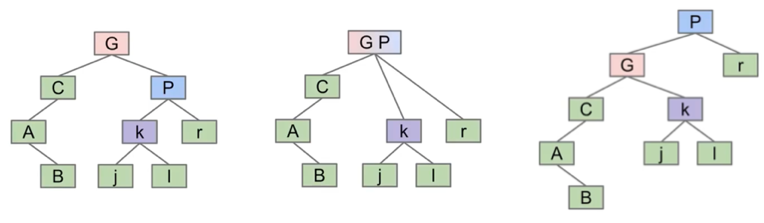
\includegraphics[width = \textwidth]{rotation.png}
	\caption{process of rotateLeft(G)}
	\label{rotation_process}
\end{figure}

\paragraph{}
Below is the code in $Java$ to implement these functions.

\begin{verbatim}

//rotateLeft
private void leftRototate(){
    //create a new node with the value of root
    Node newNode = new Node(this.value);

    //new node's left child -> root's left child
    newNode.left = this.left;

    //new node's right child -> root's right child's left child
    newNode.right = this.right.left;

    //set root's value to its right child's value
    this.value = right.value;

    //root's right child -> it's right child
    right = right.right;

    //root's left child -> the new node
    left = newNode;
}


//rotateRight
private void rightRotate(){
    //create a new node with the value of root
    Node newNode = new Node(this.value);

    //new node's right child -> root's right child
    newNode.right = this.right;

    //new node's left child -> root's left child's right child
    newNode.left = this.left.right;

    //set root's value to its left child's value
    this.value = this.left.value;

    //root's left child -> it's left child
    this.left = this.left.left;

    //root's right child -> the new node
    right = newNode;
}

\end{verbatim}

\paragraph{}
Tree rotation is used to change the tree's shape and, in particular, to decrease its height by moving smaller subtrees down and larger subtrees up, resulting in improved performance of many tree operations.

Since applying rotation won't affect the in-order of the tree, a BST is still a BST after rotation.

\subsubsection{Unbalanced Situation}\label{unbalanced_situation}

\begin{definition}
    In a binary tree, the balance factor of node X ($BF(X)$) is defined as the height difference of its two child sub-trees.
\end{definition}

\begin{definition}
    An unbalanced tree contains a node $X$ with $|BF(X)| > 1$.
\end{definition}

\paragraph{}
Though there are all kinds of unbalanced trees, there are only 4 kinds of unbalanced situations. (shown as figure~\ref{unbalance} below)

\begin{figure}[htbp]
    \centering
	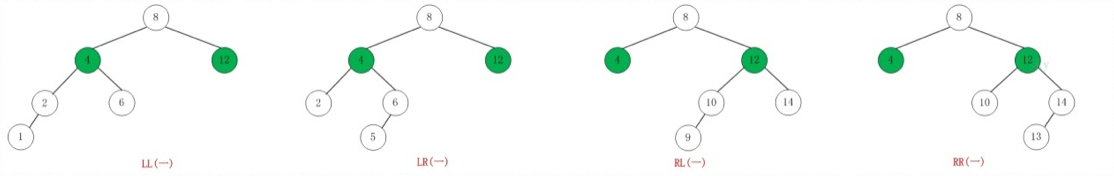
\includegraphics[width = \textwidth]{unbalance.png}
	\caption{unbalanced situations(LL LR RL RR)}
	\label{unbalance}
\end{figure}

\paragraph{}
With tree rotation, we can fix all these kinds of unbalanced trees into balanced trees:

It turns into a balanced tree by applying rotateRight() to the root node in LL.

It turns into a balanced tree by applying rotateLeft() to left child(now it becomes LL) and then rotateRight() to the root node in LR.

It turns into a balanced tree by applying rotateRight() to right child(now it becomes RR) and then rotateLeft() to the root node in RL.

It turns into a balanced tree by applying rotateLeft() to the root node in RR.

\paragraph{}
What AVL tree does is detect whether an unbalance situation takes place when adding or deleting data. If it does happen, then fix them throw rotation.

\subsubsection{Performance}

\paragraph{}
AVL tree is an absolutely balanced binary search tree, which can ensure efficient query time complexity, that is, $O(\log{N})$. However, the performance is very low to do some structural modification operations on the AVL tree, such as: maintaining its absolute balance when inserting, and the number of rotations is relatively large. When deleting, letting the rotation continue to the root position is possible.


\newpage


\subsection{B-tree}

\paragraph{}
Besides using tree rotation, another idea to implement a self-balancing tree is using some ingenious construction. B-tree follows this idea and has a good performance.

\subsubsection{Naive Approach}

\paragraph{}
Consider when the balance situation would be broken. When a new leaf node is added to the tree, the height of one subtree will increase, which means the balance may be ruined.

To avoid this, the tree just put the data in our existing node instead of adding a new leaf node to store data.

For example, in figure~\ref{naive_b_example} below, a complete BST is on the left side. To insert 17 into the tree, we put it into the node containing 16 directly. To insert 18, we put it into the node containing 16 and 17.

\begin{figure}[htbp]
    \centering
	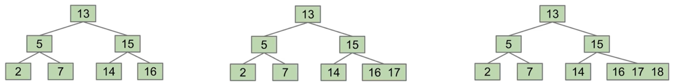
\includegraphics[width = \textwidth]{naive_b_example.png}
	\caption{a naive idea of B-tree}
	\label{naive_b_example}
\end{figure}

\paragraph{}
The tree uses a list as a node to solve the problem. It's useful when the list is short. Binary search can be applied to the tree, and by iterating the list, it's easy to find the data stored in the list node.

But when the list gets longer, this approach is not efficient enough. The time taken to iterate the list is way much than the time for using binary search to find the list node, so the tree approximately degenerates into a linked list.(figure~\ref{naive_b_problem})

\begin{figure}[htbp]
    \centering
	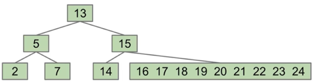
\includegraphics[width = \textwidth]{naive_b_problem.png}
	\caption{a naive B-tree with a long list}
	\label{naive_b_problem}
\end{figure}

\subsubsection{Solution}

\paragraph{}
A limitation to the maximum list length is set to avoid the degeneration problem.

For example, if the maximum length of the list of the tree in figure~\ref{b_first} is 3, then the list has to be shortened. 

\paragraph{}
In B-tree, the data in the middle of the list(the left middle is the length is even) would be moved to the parent node of the list node.

For instance, the tree in figure~\ref{b_first} would be transformed into the tree in figure~\ref{b_second}.

But the result isn't satisfying. In the second tree, 17's child node is a list containing $16,18,19$, which has numbers both larger and smaller than it. This way, no efficient algorithm can be used to search data here.

\paragraph{}
While moving the data in the middle, B-tree also split the list from that position.

Thus, the tree in figure~\ref{b_second} would turn into the tree in figure~\ref{b_third}. Now that data are put in order, data in this tree can be searched using a combination of binary and linear search.

\begin{figure}[htbp]

    \centering

    \begin{minipage}{0.3\linewidth}
        \centering
        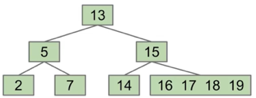
\includegraphics[width = \textwidth]{b_first.png}
        \caption{bad form}
        \label{b_first}
    \end{minipage}
    \begin{minipage}{0.3\linewidth}
        \centering
        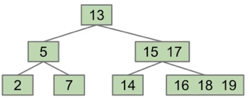
\includegraphics[width = \textwidth]{b_second.png}
        \caption{try to change}
        \label{b_second}
    \end{minipage}
    \begin{minipage}{0.3\linewidth}
        \centering
        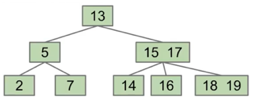
\includegraphics[width = \textwidth]{b_third.png}
        \caption{good form}
        \label{b_third}
    \end{minipage}

    \caption{B-tree transforming}
\end{figure}


\paragraph{}
A B-tree of order\footnote{The order of the tree represents the maximum number of children a tree's node could have. Through property~\ref{property_ktok+1}, if the maximum length of list of a B-tree is $m$, the order of the tree is also $m$}
$m$ has 4 properties according to its operation form.

\begin{property}
    Every node except the root must contain at least $m/2-1$ keys. The root may contain a minimum of 1 key.
\end{property}

\begin{property}
    All nodes may contain at most $m - 1$ keys.
\end{property}

\begin{property}\label{property_samedistance}
    All leaves must be the same distance from the source.
\end{property}

\begin{property}\label{property_ktok+1}
    A non-leave node with $k$ items must have exactly $k+1$ children.
\end{property}

\paragraph{}
There are 2 situations to consider while deleting data from a B-tree: non-leaf node and leaf node. It's relatively complicated. The web \href{https://www.programiz.com/dsa/deletion-from-a-b-tree}{here} explains the logic of B-tree deletion well.

\subsubsection{B+ tree}\label{b+}

\paragraph{}
Though B-tree is good enough, B+ tree is invented to adapt the usage in database better.

\paragraph{}
A B+ tree has all properties that a B-tree has, but there are several differences between the structure of a B-tree and a B+ tree:

\subparagraph{}
In B+ tree, only leaf nodes store actual data. Therefore, a B+ tree can store more keys per node than a B-tree if they have the same order. This is important since the capability of pages is fixed for hardware. B+ tree stores more keys in a page\footnote{For B-tree and B+ tree which are used in database, a node corresponds to a page(see~\ref{application})}
than b-tree so that it can store more data with the same layers.

What's more, since all data are stored in leaf nodes in a B+ tree, and all leaves are the same distance from the source(property~\ref{property_samedistance}), so the time it takes to search different data is similar, which is more fair compares to B-tree.

\subparagraph{}
The leaves are not connected with each other on a B-tree, whereas they are connected on a B+ tree. Thus, a B+ tree can deal with range queries more efficiently. In B+ tree, after finding the beginning data, the rest data can be obtained through the extra link. Contrastingly, continuous data may not be stored in the continuous memory area, which means it's hard to respond to a range query.


\subsubsection{Performance}
If the order of the B-tree is large, when there is little data, the tree is similar to a linked list, which would be very slow. With a reasonable order, B-tree is fast. For a B-tree of order $m$ with $N$ nodes, inserting or searching data takes between $\log_{m-1}N$ to $\log_{m/2}N$ times of comparison.


\newpage


\subsection{Red Black tree}

\paragraph{}
Red Black tree(RBtree) is a kind of self-balancing tree that also uses tree rotation(\ref{rotation}). Still, it has some other properties, so less time is needed to maintain balance when inserting/deleting data. However, it's not as balanced as the AVL tree, so a longer time is required to respond to queries.

\paragraph{}
There are two kinds of nodes in a RBtree: red node and black node. All RBtree types correspond to B-tree; a red node and its parent node(which must be a black node) can be seen as 'glued', which corresponds to list nodes in B-tree.

\subsubsection{Left Leaning Red Black tree}

\paragraph{}
There are many variations of RBtree, and left-leaning RBtree(LLRB) is one of them. It's easier to implement and has similar performance compared to RBT.

\begin{property}\label{BRT1on1}
    1-1 correspondence with 2-3 trees\footnote{A 2-3 tree means a B-tree of order 3}.
\end{property}

\begin{property}
    No node has 2 red links.
\end{property}

\begin{property}
    Every path from the root to leaf has same number of black links (because 2-3 trees have same number of links to every leaf).
\end{property}

\begin{property}
    Height is no more than 2x height of corresponding 2-3 tree.
\end{property}

\paragraph{}
Since property~\ref{BRT1on1}, by inserting into a 2-3 tree and converting it to let the tree has properties above, the result of inserting into LLRB can be obtained. However, this is stupid since there is no point in spending extra time to transform a usable 2-3 tree into a LLRB. So the proper method is to insert into the LLRB the same as a normal BST and then use rotations to fix its 1-1 map to 2-3 tree.

\paragraph{}
Here are the tasks that need to be done when inserting into a LLRB:

\subparagraph{}\label{LLRB_insert}
In 2-3 trees, data always be added into a leaf node, so the colour of the link added to LLRB should always be red.

\subparagraph{}
According to the name, a red link should never appear on the right side. A rotation should be applied to maintain the LLRB property.

However, if the node has two red links, it needs to be allowed to exist for a while.

\subparagraph{}
If there are 2 left red links, it corresponds to a list with a length of 4. After rotating to create a tree with two red links, flipping the colours of all edges touching the node.

\paragraph{}
Though it seems complex to fix the format, only 3 if-sentences are needed to update an AVL tree to an LLRB.

\begin{verbatim}

private Node put(Node h, Key key, Value val) {
    if (h == null) {
        return new Node(key, val, RED);
    }

    int cmp = key.compareTo(h.key);

    if (cmp < 0) {
        h.left  = put(h.left,  key, val);
    }

    else if (cmp > 0) {
        h.right = put(h.right, key, val);
    }
    else {
        h.val = val;
    }

    if (isRed(h.right) && !isRed(h.left)) {
        h = rotateLeft(h);
    }
    if (isRed(h.left) && isRed(h.left.left)) {
        h = rotateRight(h);
    }
    if (isRed(h.left) && isRed(h.right)) {
        flipColors(h);
    } 

return h;

}
\end{verbatim}

\paragraph{}
Because a left-leaning red-black tree has a 1-1 correspondence with a 2-3 tree and will always remain within 2x the height of its 2-3 tree, the runtimes of the operations will take $\log{N}$ time.

\subsubsection{Normal RBtree}

\paragraph{}
An LLRB can only have one red link per node, corresponding to a 2-3 tree. In a normal RBtree, each node can have 2 red links, corresponding to a 2-3-4 tree\footnote{A 2-3-4 tree means a B-tree of order 4}.

\paragraph{}
Here are the properties that an RBtree should have:

\begin{property}
    The root node of RBtree is black.
\end{property}

\begin{property}
    The leaf nodes\footnote{The leaf node in RBtree is slightly different, it refers to the lowest empty nodes (external nodes)}
    are all black.
\end{property}

\begin{property}\label{RBt_property}
    Red nodes' children and parent are black nodes.
\end{property}

\paragraph{}
Classification by the node case after the conversion of RBtree to B-tree can be made use of the equivalence property of the 2-3-4 tree and red-black tree.(see figure~\ref{RBtree_Classification})

\begin{figure}[htbp]
    \centering

    \begin{minipage}{0.49\linewidth}
        \centering
        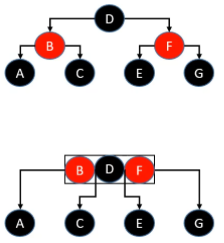
\includegraphics[height = 90 pt]{rbr.png}
        \caption{red black red}
        \label{rbr}
    \end{minipage}
    \begin{minipage}{0.49\linewidth}
        \centering
        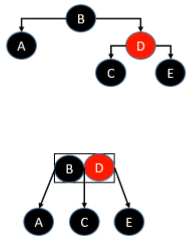
\includegraphics[height = 90 pt]{br.png}
        \caption{black red}
        \label{br}
    \end{minipage}

    \begin{minipage}{0.49\linewidth}
        \centering
        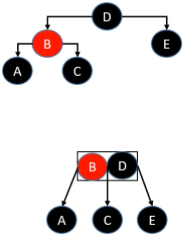
\includegraphics[height = 90 pt]{rb.png}
        \caption{red black}
        \label{rb}
    \end{minipage}
    \begin{minipage}{0.49\linewidth}
        \centering
        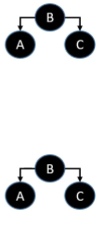
\includegraphics[height = 90 pt]{b.png}
        \caption{black}
        \label{b}
    \end{minipage}

    \caption{4 situations of RBtree node}
    \label{RBtree_Classification}
\end{figure}

\paragraph{}
Same as LLRB, the colour of a new node being inserted is red.(see \ref{LLRB_insert})

Considering how to insert a new node into the tree in figure~\ref{RBt_example} makes it easier to understand how an RBtree maintains its properties.

\begin{figure}[htbp]
    \centering

    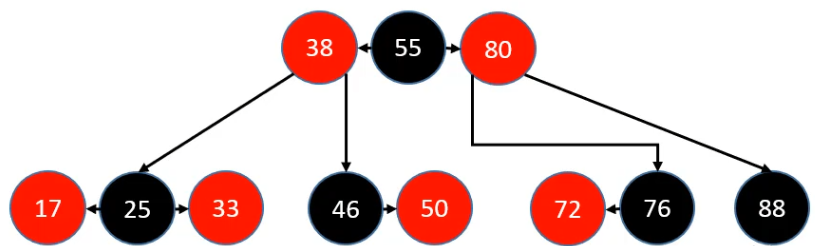
\includegraphics[height = 50 pt]{RBtree.png}
    \caption{a RBtree}
    \label{RBt_example}
\end{figure}

\paragraph{}
The RBtree in figure~\ref{RBt_example} contains all the previously classified situations. 12 places in this tree can insert new nodes. Among them, 4 situations don't require any further operation to maintain the properties(cases shown in figure~\ref{RBt_accepted})

\begin{figure}[htbp]
    \centering

    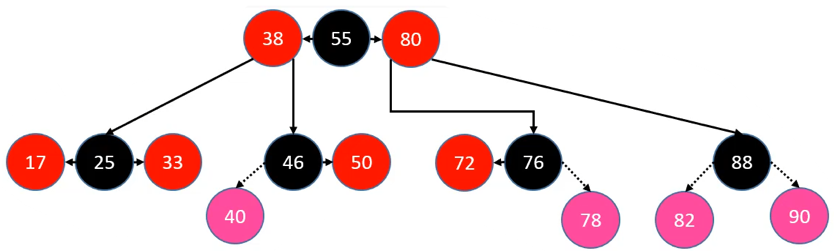
\includegraphics[height = 50 pt]{RBt_accepted.png}
    \caption{4 places that don't need further operation}
    \label{RBt_accepted}
\end{figure}

\paragraph{}
8 situations do not satisfy the property of red-black tree~\ref{RBt_property}, and 4 situations on the left belong to the overflow situation of B-tree nodes (a 4-order B-tree node can store a maximum of 3 numbers, and these 4 cases already have 3 numbers, and another one is inserted, which beyond the capacity range of the 4-order B-tree node). These 8 cases require additional processing. (figure~\ref{RBt_rejected})

\begin{figure}[htbp]
    \centering

    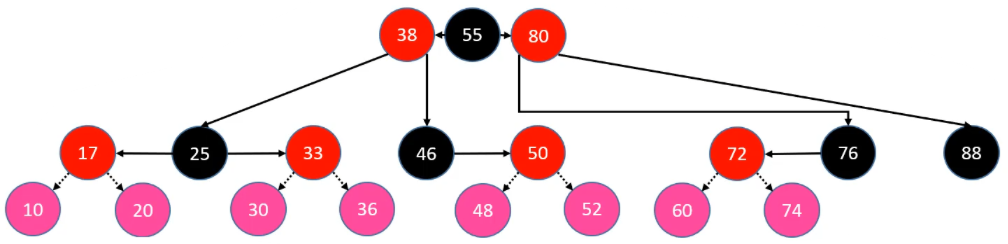
\includegraphics[height = 50 pt]{RBt_rejected.png}
    \caption{other places that need further operation}
    \label{RBt_rejected}
\end{figure}

\paragraph{}
The situations can be named by their unbalance situations(see~\ref{unbalanced_situation}). For example, for the tree in figure~\ref{RBt_rejected}, insert node 10 or 60 forms LL; insert node 36 or 52 forms RR; insert node 20 or 74 forms LR; insert node 30 or 48 forms RL

\paragraph{}
For cases without overflow:

To fix LL/RR, dye parent black and grand red.

To fix LR/RL, dye inserted node black and grand red.

Then apply rotation mentioned in~\ref{rotation}.

\paragraph{}
For cases with overflow:

Dye parent and uncle black and grand red.

\subsubsection{Performance}

\paragraph{}
RBtree ensures that the longest path is not more than twice the shortest path, so it is approximately balanced (the shortest path is an all-black node, the longest path is a red node and a black node, and when the path from the root node to the leaf node has the same black node, the longest path is exactly twice the shortest path).

RBtree's search, insert, and delete operations are all $O(\log N)$ in time complexity.

\newpage


\subsection{Applications}\label{application}

\subsubsection{AVL tree and Red Black tree}
\paragraph{}
An AVL tree is suitable when a data structure that is query efficient and ordered and the number of data is static is needed, but a system that changes frequently is not a good fit.

In real life, most data in memory changes frequently. RBtree is used to store data there mostly\footnote{Many ADTs like hashmap, treemap, and treeset use RBtree to store data since RBtree can significantly shorten the searching operation time for any data size.}.
For database system, tree structure will fewer layers are better since hard disk IO is too expensive.(see B-tree and B+ tree~\ref{b_application})

\paragraph{}
As a result, though AVL tree can solve the unbalance problem, it's too slow to be used. It's more common for AVL tree to appear in data structure course book to let students understand the idea and commemorate the progress from nothing to something.

Though RBtree is not as balanced as AVL tree, it has better overall performance, which means in most situations, an RBtree would be used rather than AVL tree.

\subsubsection{B-tree and B+ tree}\label{b_application}

\paragraph{}
When data is little, Red Black tree is faster than B-tree. But storing a large amount of data on hard disks makes putting a page into memory time-consuming, so using fewer pages is better. B-tree is suitable for doing this. The order of B-tree should be as large as possible to get fewer layers, so each node corresponds to a page. This way, only a few pages need to be mentioned to deal with a query. For instance, within 4 pages, an element would be found among $6.2 * 10^{10}$ elements.

\paragraph{}
However, most databases are now using B+ tree, since it has some improvements compared to B-tree.

The leaves are not connected on a B-tree, whereas they are connected on a B+ tree. Thus, a B+ tree can deal with range queries more efficiently. In B+ tree, after finding the beginning data, the rest data can be obtained through the extra link. Contrastingly, continuous data may not be stored at continuous memory area, which means it's hard to respond to a range query.


\newpage


\subsection{comparison}

\paragraph{}
Though the time complexity of these trees can be calculated, it's more visualized to run the code and see the result. And in real life, sometimes the result may differ from the theoretical result.

By searching the implementations online and writing a program to compare the time these trees needed to insert and search data, the result in appendix~\ref{result} came out.

\begin{figure}[htbp]
    \centering

	\begin{minipage}{0.49\linewidth}
		\centering
		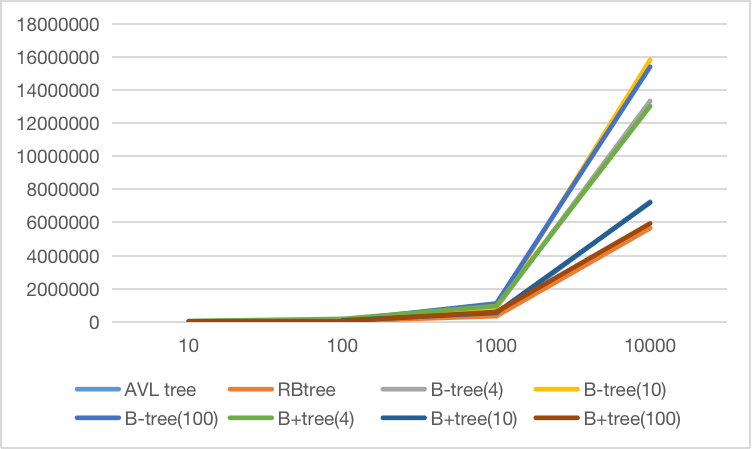
\includegraphics[width = \textwidth]{result1.png}
	\end{minipage}
	\begin{minipage}{0.49\linewidth}
		\centering
		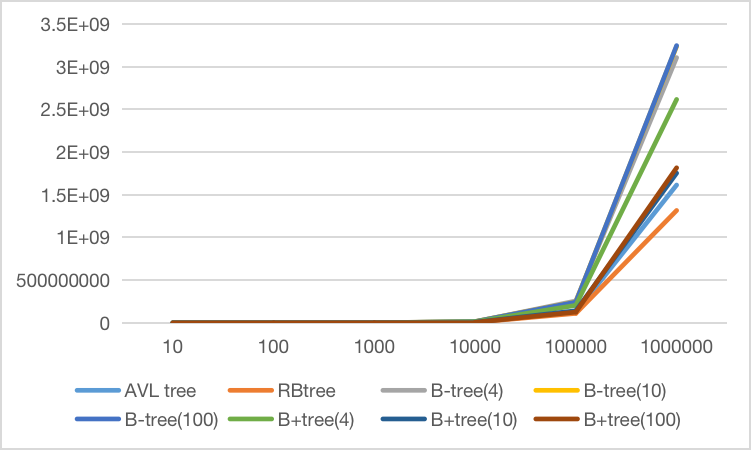
\includegraphics[width = \textwidth]{result2.png}
	\end{minipage}

    \caption{data size -- insert time(ns)}
    \label{data1}
\end{figure}

\begin{figure}[htbp]
    \begin{minipage}{0.49\linewidth}
		\centering
		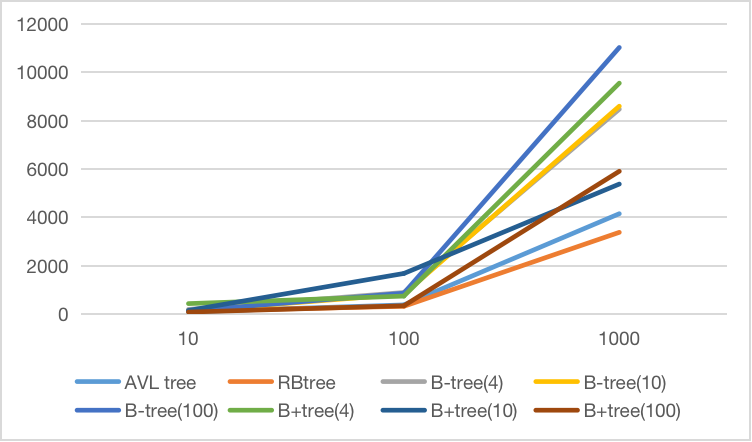
\includegraphics[width = \textwidth]{result3.png}
	\end{minipage}
    \begin{minipage}{0.49\linewidth}
		\centering
		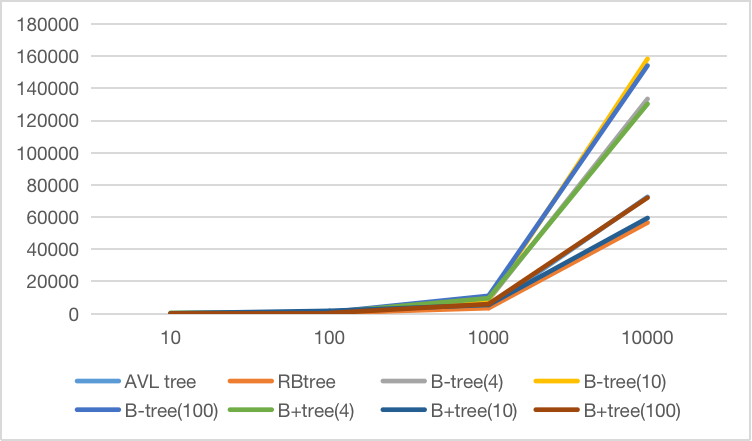
\includegraphics[width = \textwidth]{result4.png}
	\end{minipage}

    \begin{minipage}{0.49\linewidth}
		\centering
		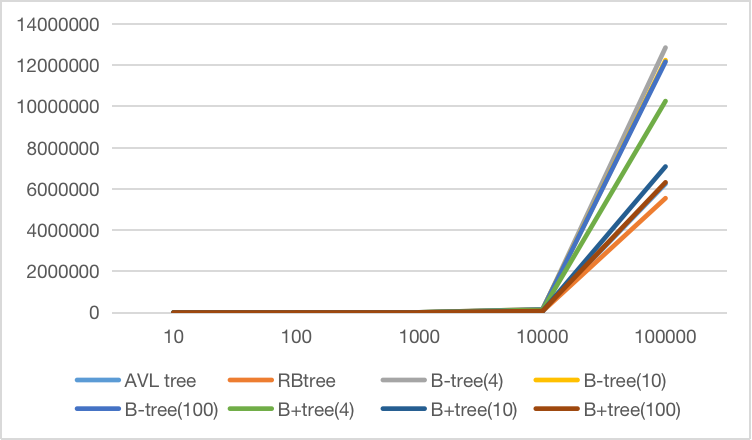
\includegraphics[width = \textwidth]{result5.png}
	\end{minipage}
    \begin{minipage}{0.49\linewidth}
		\centering
		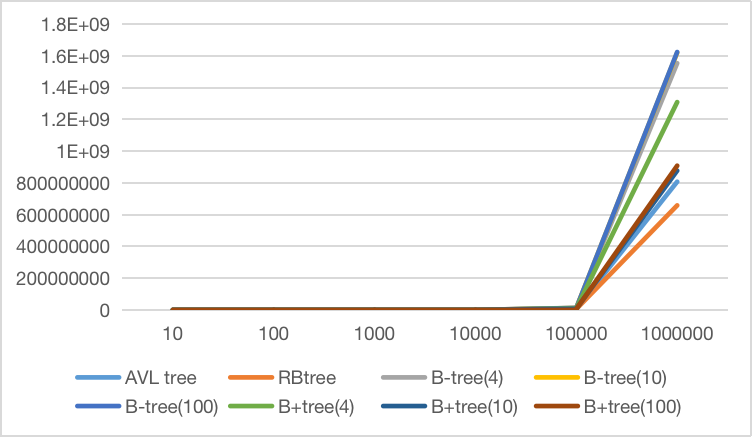
\includegraphics[width = \textwidth]{result6.png}
	\end{minipage}

    \caption{data size -- query time(ns)}
    \label{data2}

\end{figure}

\paragraph{}
The line charts in figure~\ref{data1} and figure~\ref{data2} are drawn by organizing the data.

\paragraph{}
From figure~\ref{data1}, when the data set is relatively small($n * 10^3$), B-tree of order 10 and B-tree of order 100 perform the worst. The difference is more significant when the data set grows larger($n * 10^5$). B-trees have the worst performance, B+ trees are better, and RBtree, faster than AVL tree, performs best. This is roughly consistent with theoretical speculation.

\paragraph{}
In figure~\ref{data2}, AVL tree and RBtree are generally still the best, B+ tree follows and B-tree is the worst. But this is different from the theory since logically AVL tree should be faster than RBtree when dealing with queries. This is probably because the optimize of the code for RBtree is better. Also, for B+ tree, the code uses array as leaf node, so binary search can be applied. But in B-tree the nodes are linked list, which means it will use linear search, which is much slower.

\paragraph{}
The code for this test can be found \href{https://github.com/yty-yang/TreeComparison.git}{here}.

\newpage
\bibliographystyle{plain}
\bibliography{reference}
\nocite{*}

\newpage

\appendix
\section{Original result of code}\label{result}
\begin{verbatim}
insert 10 nodes to AVL tree:             10667 ns
insert 10 nodes to RBtree:               19292 ns
insert 10 nodes to B-tree of order 4:    24000 ns
insert 10 nodes to B-tree of order 10:   17334 ns
insert 10 nodes to B-tree of order 100:  13833 ns
insert 10 nodes to B+ tree of order 4:   22583 ns
insert 10 nodes to B+ tree of order 10:  31459 ns
insert 10 nodes to B+ tree of order 100: 12541 ns
fast <------------insert------------> slow
AVL B+(100) B(100) B(10) RBt B+(4) B(4) B+(10) 
search in AVL tree:            3500 ns
search in RBtree:              3792 ns
search in B-tree of order 4:   5625 ns
search in B-tree of order 10:  2250 ns
search in B-tree of order 100: 2000 ns
search in B+tree of order 4:   3917 ns
search in B+tree of order 10:   1750 ns
search in B+tree of order 100: 1208 ns
fast <------------search------------> slow
B+(100) B+(10) B(100) B(10) AVL RBt B+(4) B(4) 

averagetime_insert:
{B(10)=12329.16, B+(100)=8404.08, B+(4)=43430.38, 
B(100)=12608.37, RBt=12471.66, B(4)=19601.28, 
AVL=9443.35, B+(10)=15146.59}
averagetime_search:
{B(10)=123.2916, B+(100)=84.0408, 
B+(4)=434.30379999999997, B(100)=126.08370000000001, 
RBt=124.7166, B(4)=196.0128, AVL=94.43350000000001, 
B+(10)=151.4659}
----------------------------------------------------
insert 100 nodes to AVL tree:             34958 ns
insert 100 nodes to RBtree:               30959 ns
insert 100 nodes to B-tree of order 4:    141916 ns
insert 100 nodes to B-tree of order 10:   80333 ns
insert 100 nodes to B-tree of order 100:  94500 ns
insert 100 nodes to B+ tree of order 4:   126542 ns
insert 100 nodes to B+ tree of order 10:  65709 ns
insert 100 nodes to B+ tree of order 100: 42875 ns
fast <------------insert------------> slow
RBt AVL B+(100) B+(10) B(10) B(100) B+(4) B(4) 
search in AVL tree:            1625 ns
search in RBtree:              1500 ns
search in B-tree of order 4:   3208 ns
search in B-tree of order 10:  2042 ns
search in B-tree of order 100: 1584 ns
search in B+tree of order 4:   1958 ns
search in B+tree of order 10:   791 ns
search in B+tree of order 100: 708 ns
fast <------------search------------> slow
B+(100) B+(10) RBt B(100) AVL B+(4) B(10) B(4) 

averagetime_insert:
{B(10)=82433.71, B+(100)=34530.4, B+(4)=168120.84, 
B(100)=86569.96, RBt=32285.04, B(4)=89461.76, 
AVL=38018.79, B+(10)=74490.4}
averagetime_search:
{B(10)=824.3371000000001, B+(100)=345.30400000000003, 
B+(4)=1681.2084, B(100)=865.6996, 
RBt=322.85040000000004, B(4)=894.6175999999999, 
AVL=380.1879, B+(10)=744.904}
----------------------------------------------------
insert 1000 nodes to AVL tree:             457375 ns
insert 1000 nodes to RBtree:               401417 ns
insert 1000 nodes to B-tree of order 4:    885834 ns
insert 1000 nodes to B-tree of order 10:   900209 ns
insert 1000 nodes to B-tree of order 100:  845959 ns
insert 1000 nodes to B+ tree of order 4:   929208 ns
insert 1000 nodes to B+ tree of order 10:  589458 ns
insert 1000 nodes to B+ tree of order 100: 424625 ns
fast <------------insert------------> slow
RBt B+(100) AVL B+(10) B(100) B(4) B(10) B+(4) 
search in AVL tree:            1916 ns
search in RBtree:              1959 ns
search in B-tree of order 4:   3291 ns
search in B-tree of order 10:  1458 ns
search in B-tree of order 100: 1750 ns
search in B+tree of order 4:   2250 ns
search in B+tree of order 10:   875 ns
search in B+tree of order 100: 416 ns
fast <------------search------------> slow
B+(100) B+(10) B(10) B(100) AVL RBt B+(4) B(4) 

averagetime_insert:
{B(10)=859769.16, B+(100)=590647.05, B+(4)=955079.98, 
B(100)=1102582.06, RBt=338150.86, B(4)=847384.17, 
AVL=415199.65, B+(10)=537789.11}
averagetime_search:
{B(10)=8597.6916, B+(100)=5906.4705, B+(4)=9550.7998, 
B(100)=11025.820600000001, RBt=3381.5085999999997, 
B(4)=8473.8417, AVL=4151.9965, B+(10)=5377.8911}
----------------------------------------------------
insert 10000 nodes to AVL tree:             9670000 ns
insert 10000 nodes to RBtree:               8590000 ns
insert 10000 nodes to B-tree of order 4:    18246166 ns
insert 10000 nodes to B-tree of order 10:   20345250 ns
insert 10000 nodes to B-tree of order 100:  19274125 ns
insert 10000 nodes to B+ tree of order 4:   15648833 ns
insert 10000 nodes to B+ tree of order 10:  10381458 ns
insert 10000 nodes to B+ tree of order 100: 7639125 ns
fast <------------insert------------> slow
B+(100) RBt AVL B+(10) B+(4) B(4) B(100) B(10) 
search in AVL tree:            1375 ns
search in RBtree:              2292 ns
search in B-tree of order 4:   5292 ns
search in B-tree of order 10:  3583 ns
search in B-tree of order 100: 3583 ns
search in B+tree of order 4:   4833 ns
search in B+tree of order 10:   3167 ns
search in B+tree of order 100: 792 ns
fast <------------search------------> slow
B+(100) AVL RBt B+(10) B(100) B(100) B+(4) B(4) 

averagetime_insert:
{B(10)=1.58285672E7, B+(100)=5938541.24, 
B+(4)=1.303157998E7, B(100)=1.541014462E7, 
RBt=5652890.43, B(4)=1.334035707E7, AVL=7253795.84, 
B+(10)=7203287.06}
averagetime_search:
{B(10)=158285.672, B+(100)=59385.4124, 
B+(4)=130315.79980000001, B(100)=154101.4462, 
RBt=56528.904299999995, B(4)=133403.5707, 
AVL=72537.9584, B+(10)=72032.8706}
----------------------------------------------------
insert 100000 nodes to AVL tree:             146884792 ns
insert 100000 nodes to RBtree:               120585791 ns
insert 100000 nodes to B-tree of order 4:    277470166 ns
insert 100000 nodes to B-tree of order 10:   255380625 ns
insert 100000 nodes to B-tree of order 100:  245922541 ns
insert 100000 nodes to B+ tree of order 4:   369338292 ns
insert 100000 nodes to B+ tree of order 10:  133651708 ns
insert 100000 nodes to B+ tree of order 100: 107554834 ns
fast <------------insert------------> slow
B+(100) RBt B+(10) AVL B(100) B(10) B(4) B+(4) 
search in AVL tree:            3125 ns
search in RBtree:              2875 ns
search in B-tree of order 4:   7791 ns
search in B-tree of order 10:  4834 ns
search in B-tree of order 100: 4041 ns
search in B+tree of order 4:   4958 ns
search in B+tree of order 10:   4166 ns
search in B+tree of order 100: 1208 ns
fast <------------search------------> slow
B+(100) RBt AVL B(100) B+(10) B(10) B+(4) B(4) 

averagetime_insert:
{B(10)=2.448318646E8, B+(100)=1.2629613555E8, 
B+(4)=2.0513267075E8, B(100)=2.4331373115E8, 
RBt=1.108997041E8, B(4)=2.5701895625E8, 
AVL=1.2480924385E8, B+(10)=1.416284334E8}
averagetime_search:
{B(10)=1.224159323E7, B+(100)=6314806.7775, 
B+(4)=1.02566335375E7, B(100)=1.2165686557500001E7, 
RBt=5544985.205, B(4)=1.28509478125E7, 
AVL=6240462.1925, B+(10)=7081421.67}
----------------------------------------------------
insert 1000000 nodes to AVL tree:             1784261125 ns
insert 1000000 nodes to RBtree:               1420085958 ns
insert 1000000 nodes to B-tree of order 4:    3438281834 ns
insert 1000000 nodes to B-tree of order 10:   3788487625 ns
insert 1000000 nodes to B-tree of order 100:  3752132584 ns
insert 1000000 nodes to B+ tree of order 4:   2927331208 ns
insert 1000000 nodes to B+ tree of order 10:  2162745500 ns
insert 1000000 nodes to B+ tree of order 100: 1330336083 ns
fast <------------insert------------> slow
B+(100) RBt AVL B+(10) B+(4) B(4) B(100) B(10) 
search in AVL tree:            9750 ns
search in RBtree:              23958 ns
search in B-tree of order 4:   73917 ns
search in B-tree of order 10:  72917 ns
search in B-tree of order 100: 44417 ns
search in B+tree of order 4:   101875 ns
search in B+tree of order 10:   5541 ns
search in B+tree of order 100: 2791 ns
fast <------------search------------> slow
B+(100) B+(10) AVL RBt B(100) B(10) B(4) B+(4) 

averagetime_insert:
{B(10)=3.2371293125E9, B+(100)=1.815506875E9, 
B+(4)=2.615794021E9, B(100)=3.246175146E9, 
RBt=1.315888708E9, B(4)=3.1055527505E9, 
AVL=1.613829729E9, B+(10)=1.7530696875E9}
averagetime_search:
{B(10)=1.61856465625E9, B+(100)=9.077534375E8, 
B+(4)=1.3078970105E9, B(100)=1.623087573E9, 
RBt=6.57944354E8, B(4)=1.55277637525E9, 
AVL=8.069148645E8, B+(10)=8.7653484375E8}
----------------------------------------------------
\end{verbatim}

\end{document}